\documentclass[12pt, oneside]{article}
 
\usepackage{graphicx}
\usepackage{hyperref}
\graphicspath{ {../Images/} }

\begin{document}
\thispagestyle{empty}
\begin{center}
\begin{minipage}{0.9\linewidth}
    \centering


    {\normalsize Project Tender\par}
    \vspace{1cm}
    {\Large Project: Project STORM\par}
{\normalsize Client: Linda Marshall\par}
    \vspace{1cm}
   {\Large Team: Team Name\par}
    {\normalsize Renaldo van Dyk (12204359)\par}
    {\normalsize Johann Dian Marx (12105202)\par}
    {\normalsize Sean Thomas Hill (12221458)\par}
    {\normalsize Andreas du Preez (12207871)\par}
    {\normalsize Shaun Meintjes (13310896)\par}
{\normalsize Department of Computer Science, University of Pretoria\par}
    \vspace{1cm}

 {\normalsize Date: May 2015}
\vspace{1cm}
    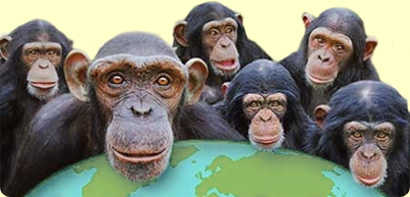
\includegraphics[scale=0.07]{example1} %Example is the name of the image

    \vspace{1cm}
    
\end{minipage}
\end{center}
\clearpage

\newpage

\section{The Team}
	\begin{enumerate}
		\item {Renaldo van Dyk (12204359)\par}
			
		\begin{itemize}		
			
\includegraphics[scale=0.1]{Renaldo} %Example is the name of the image		
			\item Interests\newline\newline
				I'm a lover of technology in general and fortunate enough to pertain to it's value. I love knowing that 
				every page of code that I write will help improve someone in their day-to-day life. I mostly favor web and 
				mobile app development and I'm also intrigued by security and privacy aspects of information technology.\newline
			\item My technical strong points:
				\begin{itemize}
				\item Java\newline
					Java programming is one of my strong points and I have been using the java language extensively for 3 years.
				\item XML\newline
					XML have been used throughout the course of 4 years in my degree. We have learned how to use it 
					in different environments and I have experimented with it in my own time by writing small android apps.
				\item Web Technologies\newline
					PHP, Javascript, HTML, JQuery, AJAX, XML are some of my well developed skills.
				\item Other Languages\newline
					Visual C\#\newline
					C++\newline
					C\newline
					ASP.net\newline
					SQL\newline
					UML\newline	
				\end{itemize}				
			\item Past experience relevant to project\newline\newline
				I have worked with web technologies for 5 years, in my field of study and in the more corporate 							environment. This experience will be crucial in the development of the web application. I have worked on some artificial intelligent applications making use of smart algorithms. I am familiar with a vast variety of data structures and how to shuffle or traverse them efficiently.\newline
			\item Non-technical strengths\newline\newline
				I am  a strong perfectionist, this means I will not attempt a project if I am not 100\% sure that I will succeed. I am driven and always do my utmost best to reach deadlines.  Some of my characteristics include:\newline 
Reliable\newline
Leader\newline
Precise\newline
Hard Working\newline
Passionate\newline
Loyal\newline
			\item What makes you want to do the project\newline\newline
				I would say web development is my strongest area of expertise. I have always loved to challenge myself 						with complex and intelligent algorithms. I will gain a lot of knowledge and experience from this 								project. I know that this project will help the CS department improve the course for future students.\newline
		\end{itemize}
		\item {Johann Dian Marx (12105202)\par}
		\begin{itemize}
			\item Photo\newline
				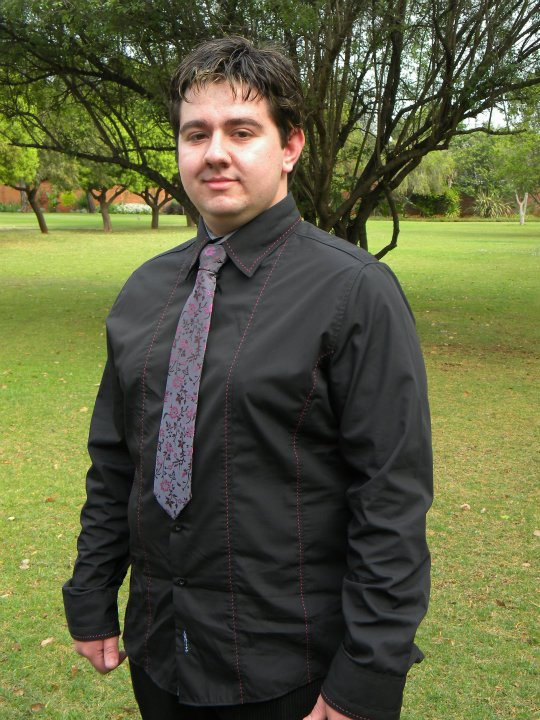
\includegraphics[scale=0.1]{Dian} %Example is the name of the image
			\item Interests\newline\newline
				My main interest is new technology. Mainly developing new software that not only enhances our daily lives,
				but also improves the safety of our data on our mobile devices.\newline
				
				I enjoy mobile development, as well as researching (and attending seminars on) security on electronic devices.
			\item Technical Skills\newline
				\begin{itemize}
				\item {\bf Java}\newline
					Not only have I been using Java for degree purposes the past 4 years, it is also my preferred coding language
					outside the confines of the university.
				\item {\bf XML}\newline
					I have used XML during my degree, and I have learned how to use it effectively.
				\item {\bf Web Technologies}\newline
					The web technologies I have acquired during my studies include, but are not limited to :
					PHP, Javascript(Used extensively by our group on the COS 301 mini-project), HTML, JQuery, AJAX, CSS.
				\item {\bf Other Languages}\newline
					Visual C\#\newline
					C++\newline
					SQL\newline
					UML\newline	
					Fortran\newline
					COBOL\newline
					Assembly\newline
					Pascal\newline
				\item {\bf Helpfull to the project}\newline
					Together with the programming skills I have acquired through the University of Pretoria, I have also done various online
					courses on Mobile Application Development(More so on Android than any other OS), as well as various courses on mobile security
					(This together with the vast amounts of research I have done on the matter).\newline
				\end{itemize}
			\item Past experience relevant to project\newline\newline
				I have worked for Corporate Companies on large projects before, which will help in the time management of the project,
				as well as the technical difficulties we might encounter.
				
				I have done some mobile development before, creating applications to be used locally between the employees of a company, which helped me 
				develop not only my knowledge of the Android environment, but also the security risks associated with sensitive information.
				
				I have worked with large groups of people, as well as individually, which I feel has prepared me for the peer programming part of the work and the individual part.\newline
			\item Non-technical strengths\newline\newline
				I have good time management skills, excel at managing groups of people, work exceptionally well under stress
				and pride myself in the work I deliver.
				I enjoy a good challenge and think this project has just enough of that to keep me going for a while. I feel the following words of Sally Hawkins are applicable here: "You only do good work when you're taking risks and pushing yourself".\newline
			\item What makes you want to do the project\newline\newline
				I am excited to work on security related projects. Working on a project for the CSIR and DPSS will help in my understanding of security measures in the Android environment, as we will have to do extensive research on the matter.
				
				Being able to say that we were part of the team that helped develop a process to keep sensitive information within the confines of the meeting space
				will also be a proud moment in any developer's student career. \newline
		\end{itemize}
		\item {Sean Thomas Hill (12221458)\par}
		\begin{itemize}
						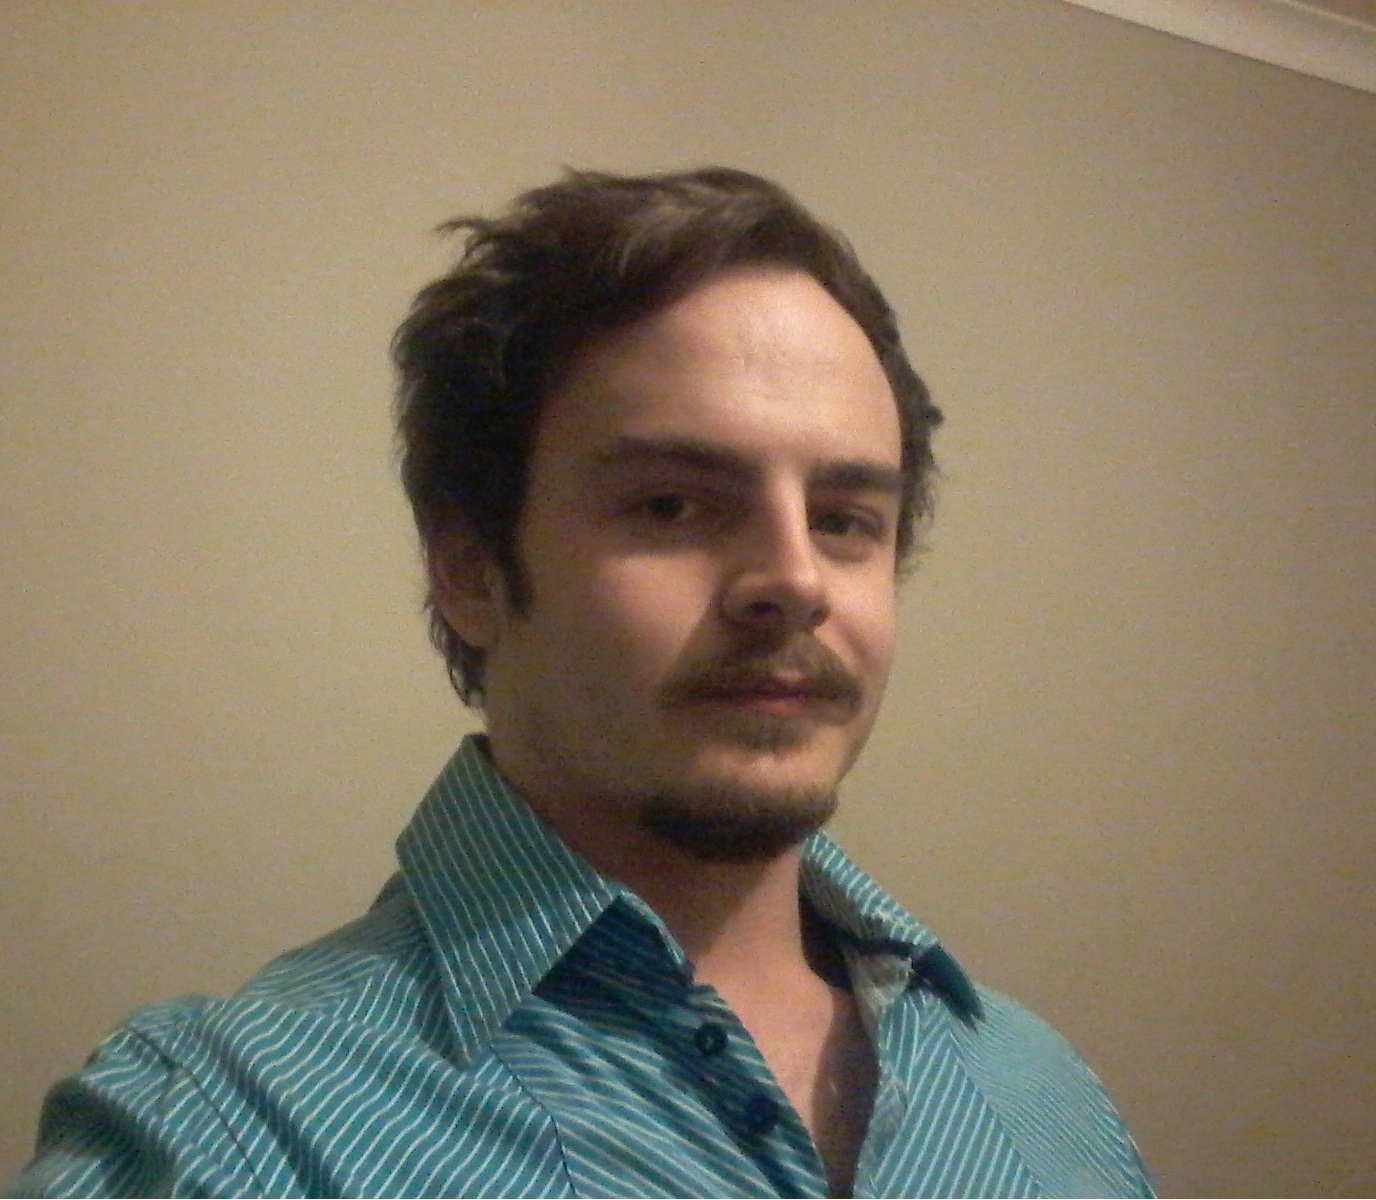
\includegraphics[scale=0.1]{Sean}
			\item Interests\newline\newline
						I'm interested in creating things that I can be proud of, and I'm excited about learning how to use a wider variety of ways to interact with the latest technology.
						Where software development is concerned I enjoy web and application development and would like to gain some more experience in mobile development as well.\newline
						
					\item Technical Skills\newline
						\begin{itemize}
						\item {\bf Java}\newline
							Three and a half years of experience in study.
						\item {\bf XML}\newline
							Extensive knowledge in xml document creation and handling of xml markup in a wide variety of coding environments as well as xml styling and template based document creation from xml documents.
						\item {\bf Web Technologies}\newline
							I am proficient in JavaScript, HTML, PHP, related database interactions and styling.
						\item {\bf Database Technologies}\newline
						MySQL, neo4j, PL/pgSQL, postGIS, db4o and mongoDB.
						\item {\bf Other Languages}\newline
							C++\newline
							Visual C\#\newline
							UML\newline	
							ASP.net\newline
							Assembly\newline
						\end{itemize}
					\item Past experience relevant to project\newline\newline
						A lot of java, database and web based development during the past four years of study.\newline
					\item Non-technical strengths\newline\newline
						I am a natural problem solver, a reliable worker and driven to complete the tasks at hand. Honesty is important to me. I am passionate about the projects we are tendering for and that means that I will do my very best to make it run perfectly. I like to keep things light and will always stay level-headed. I work well under pressure.\newline
					\item What makes you want to do the project\newline\newline
						The entire group has experience in all the technologies related with this project, we're sure we can do a fantastic job
						with it. 
				\end{itemize}
		\item {Andreas du Preez (12207871)\par}
		\begin{itemize}

				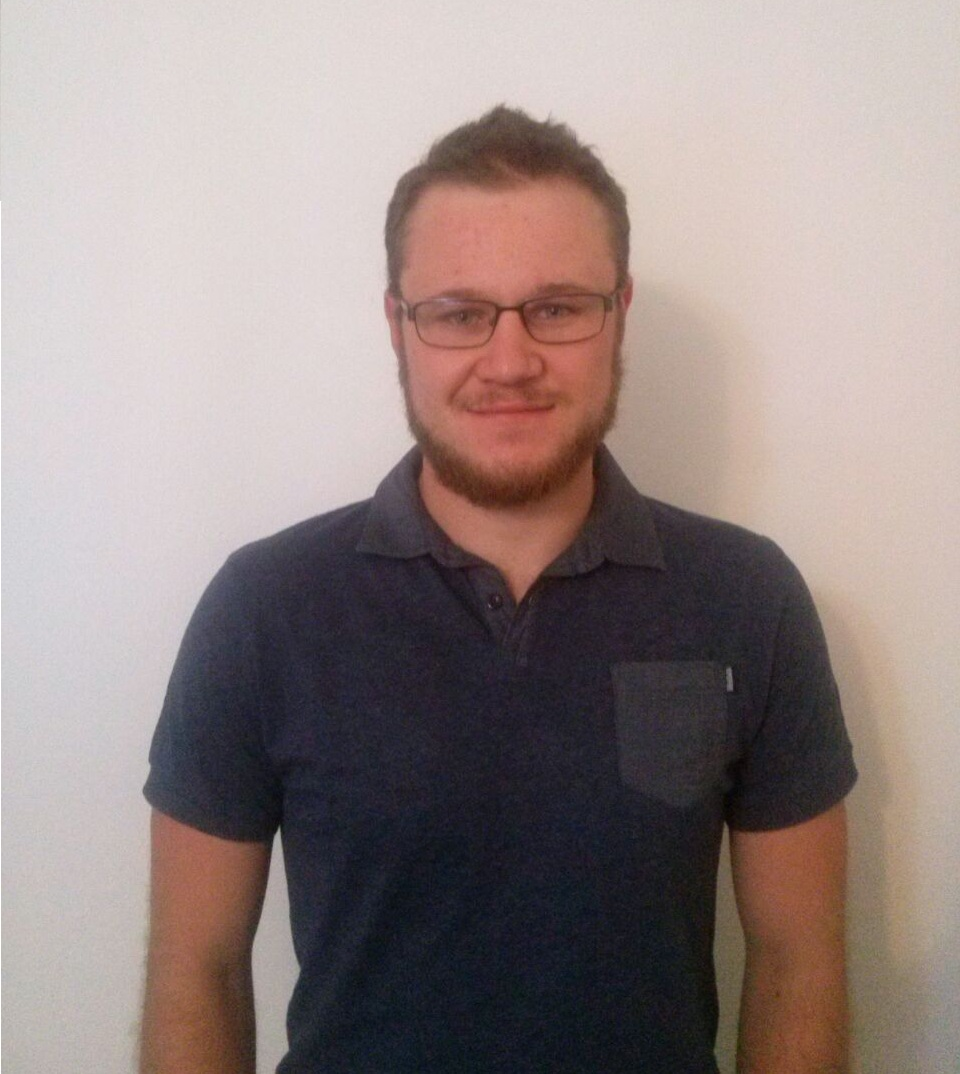
\includegraphics[scale=0.1]{Andreas} %Example is the name of the image
			\item Interests\newline\newline
				Information Technology has always been my main focus in life and I enjoy every challenge it throws at me.
				I love the fact that technology is constantly developing and I believe mobile software is a bright future for IT. 
				I take pride in my work as a software developer and wish for the users using my software the same level of enjoyment I get when programming it.\newline
			\item Technical Skills\newline\newline
			Programming languages that I've studied and have used for 4 years include:
								\begin{itemize}
								\item Java\newline
								\item C\#\newline
								\item C++\newline
								\item C\newline
								\item Markup Languages\newline
									Such as XML, HTML, XHTML, DTD, XSLT, XPath and TeX.
								\item Web Development Coding\newline
									Such as PHP, Javascript, CSS, AJAX, jNode and ASP.NET. Also I'm busy studying a variety of the World Wide Web RFC standards.
								\item Database Coding\newline
									Such as SQL, MySQL, MongoDB.
								\item Delphi\newline
								\item Assembly\newline
								\end{itemize}	
			\item Past experience relevant to project\newline\newline
				I have developed a few Android apps for personal use. I am experienced in Android software development and would love to gain professional experience. Mobile development mainly consist of Java coding, and Java is my favorite language.\newline
			\item Non-technical strengths\newline\newline
				I love a good challenge. I will walk the extra mile to complete that challenge and I won't allow anything
				to stand in my way of a project's success.\newline
			\item What makes you want to do the project\newline\newline
				I believe that networking and mobile development is the future for IT. I enjoy the concept of computers communicating with each other and wish to partake in the development of it.\newline
		\end{itemize}
		\item {Shaun Meintjes (13310896)\par}
		\begin{itemize}
				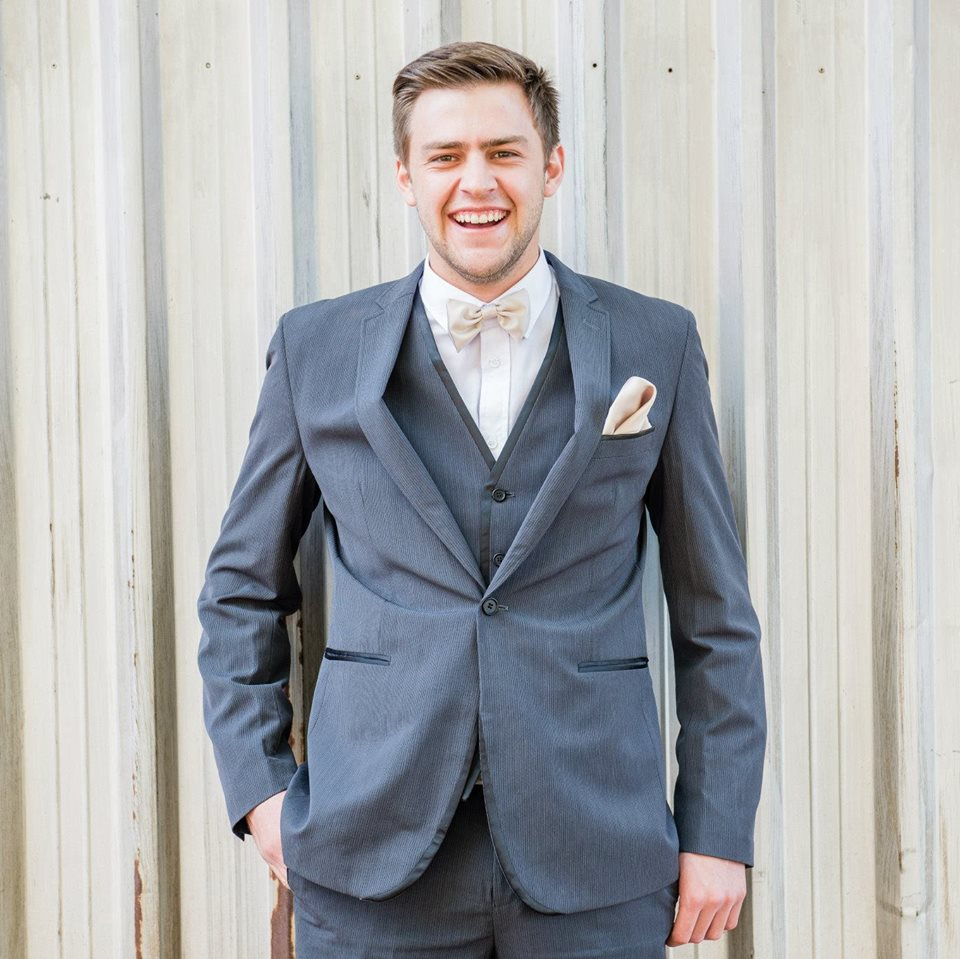
\includegraphics[scale=0.1]{Shaun} %Example is the name of the image
			\item Interests\newline\newline
				I have an interest in technology and new software that makes our daily lives easier and fun. I love to 						develop and create new things. I enjoy a challenge and then succeeding in the end. I enjoy web and 						mobile development, as well as writing systems for statistics and finances.\newline
			\item Technical Skills\newline
				\begin{itemize}
				\item {\bf Java}\newline
					Java is the language I enjoy most. I have been using Java for the past 4 years.
				\item {\bf XML}\newline
					I have used XML during my degree, and I have learned how to use it effectively.
				\item {\bf Web Technologies}\newline
					PHP, Javascript, HTML, JQuery, AJAX, XML are some of the skills that I have acquired.
				\item {\bf Other Languages}\newline
					Visual C\#\newline
					C++\newline
					C\newline
					SQL\newline
					UML\newline	
					Fortran\newline
					COBOL\newline
					Assembly\newline
				\end{itemize}
			\item Past experience relevant to project\newline\newline
				I have worked for big corporate companies to help make their processes better and faster, by writing 						certain small programs to achieve big results. This included databases, statistics, macros, XML, Java and 						web-development. I have used web-development during my degree and I have learned all of the 							languages above during my studies. I have done some mobile app development during my second year of study.\newline
			\item Non-technical strengths\newline\newline
				I am very motivated and will always strive to reach my goals in time. I set personal goals to help achieve 						the goals of the project. I am a fast learner, a good listener and I will always help other team members 						where I can. I have a healthy balance between perfectionism and time management. I am honest, a hard 						worker and loyal. I enjoy a challenge that I can learn from, to broaden my knowledge. I have good 							general knowledge and I am not afraid to take the lead on a project.\newline
			\item What makes you want to do the project\newline\newline
				I enjoy doing mobile-development and web-development. This project has a mixture of mobile-							development and web-development. This project will be a challenge, but it will be very interesting. I am 						looking forward to see software as well as an application like STORM. I would love to be part of the 							development of such an application and software.\newline
		\end{itemize}
	\end{enumerate}
	
\section{Project Execution}
	\subsection{Development Methodology}
		We will be working with the waterfall methodology, as this is a fairly linearizable project.
	\subsection{How to keep the client informed about the status of the project}
		Bi-weekly meetings will be scheduled with the client to discuss progress of the project, potential problems and any further arrangements. Furthermore we will communicate via email for any urgent queries or information needing to reach the client. More urgent matters can be discussed in person seeing that the client is on campus. 
	\subsection{Initial ideas on solving some of the technical challenges}
		Fill in later...
	\subsection{Technologies we intend to use for the project}
		Seeing that the application will be deployed on a web server some web technologies will have to be considered.
		It is also important that we are comfortable with the technologies that we choose thus we have considered the following:\newline
		PHP - As server side language\newline
		HTML5 - As web front end (includes CSS3 for styling)\newline
		Javascript - As client side language and communications with the server (includes AJAX, JQuery and JSON)
		WEBSTORM - As IDE for development.
		Mongoose - This can be used as a database for storing student information
	\subsection{What the client will receive from us at the end of the project}
		Fill in later...
	\subsection{Etc.}
		We are very excited to start working on project STORM and we'll certainly not let you down.

\end{document}
